\documentclass[tikz,border=10pt]{standalone}
\usepackage{tikz}
\usetikzlibrary{arrows.meta, positioning, fadings, shapes.arrows}

\begin{document}
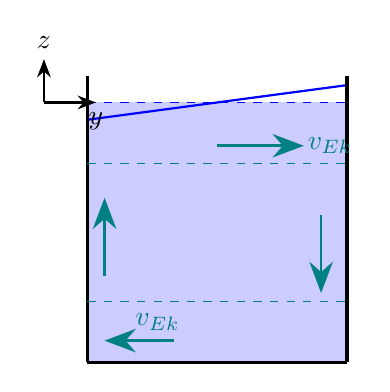
\begin{tikzpicture}[scale=1.1, >=Stealth]

\newcommand{\tikzCircleXLabel}[4]{
  % #1 = x, #2 = y, #3 = color, #4 = label
  \draw[thick, #3] (#1,#2) circle (0.2);
  \draw[thick, #3] (#1,#2) -- ({#1+0.141},{#2+0.141});
  \draw[thick, #3] (#1,#2) -- ({#1-0.141},{#2+0.141});
  \draw[thick, #3] (#1,#2) -- ({#1+0.141},{#2-0.141});
  \draw[thick, #3] (#1,#2) -- ({#1-0.141},{#2-0.141});
  \node[text=#3] at ({#1+0.9},{#2}) {#4};
}
\newcommand{\tikzCircleDotLabel}[4]{
  % #1 = x, #2 = y, #3 = color, #4 = label
  \draw[thick, #3] (#1,#2) circle (0.2);
  \fill[#3] (#1,#2) circle (2pt);
  \node[text=#3] at ({#1+0.55},{#2}) {#4};
}


% make another part of the figure below the part above:
\begin{scope}[yshift=-4.6cm]

    % draw three vertical lines representing the sea surface height

    \fill[blue!20] (0,-3) rectangle (3,0);
    \draw[dashed, blue] (0,0) -- (3,0.0) node[midway, above]{};
    \draw[thick, blue] (0,-0.2) -- (3,0.2) node[midway, above]{};
    \draw[very thick, black] (0,-3) -- (3,-3) node[midway, above]{};
    \draw[very thick, black] (0,0.3) -- (0,-3) node[midway, above]{};
    \draw[very thick, black] (3,0.3) -- (3,-3) node[midway, above]{};
    % add a hatched region beneath this to indicate sea floor better:
    \draw[dashed, teal] (0,-0.7) -- (3,-0.7) node[midway, above]{};
    % thick teal arrow pointing down from the middle of the line at x=1.5 z=-0.3
    \draw[thick, teal, -{Stealth[scale=1.5]}, line width=1pt] (1.5,-0.5) -- (2.5,-0.5) node[midway, right] {$\ \ \ \ v_{Ek}$};

    % ekman flow to left:
    \draw[thick, teal, -{Stealth[scale=1.5]}, line width=1pt] (1,-2.75) -- (0.2,-2.75) node[midway, above] {$\ \ \ \ v_{Ek}$};

    \draw[thick, teal, -{Stealth[scale=1.5]}, line width=1pt] (0.2,-2.0) -- (0.2,-1.1) node[midway, above] {};

    \draw[thick, teal, -{Stealth[scale=1.5]}, line width=1pt] (2.7,-1.3) -- (2.7,-2.2) node[midway, above] {};

    % dashed line at bottom:
    \draw[dashed, teal] (0,-2.3) -- (3,-2.3) node[midway, above]{};

    % now draw the same thing from above:
    % small axes indicating x and y directions:
    \draw[->, thick] (-0.5,0) -- (0.1,0) node[below] {$y$};
    \draw[->, thick] (-0.5,0) -- (-0.5,0.5) node[above] {$z$};

\end{scope}

%
\end{tikzpicture}
\end{document}
